% Copyright 2002-2023 The University of Maryland Baltimore County (UMBC)
% 1000 Hilltop Circle, Baltimore, Maryland, 21250, USA
% https://www.csee.umbc.edu/

\documentclass[letter,11pt]{article}
\usepackage[breaklinks]{hyperref}
\hypersetup{
    bookmarks=true,         % show bookmarks bar?
    unicode=false,          % non-Latin characters in Acrobat’s bookmarks
    pdftoolbar=true,        % show Acrobat’s toolbar?
    pdfmenubar=true,        % show Acrobat’s menu?
    pdffitwindow=false,     % window fit to page when opened
    pdfstartview={XYZ null null 1.00},    % disable zoom
    pdftitle={Homework 5},    % title
    pdfauthor={Richard Zak},     % author
    pdfsubject={UMBC CMSC104 Problem Solving and Computer Programming},   % subject of the document
    pdfkeywords={Computer Science, Programming, Problem Solving, CSEE}, % list of keywords
    pdfnewwindow=true,      % links in new PDF window
    colorlinks=false,       % false: boxed links; true: colored links
    linkcolor=red,          % color of internal links (change box color with linkbordercolor)
    citecolor=green,        % color of links to bibliography
    filecolor=magenta,      % color of file links
    urlcolor=cyan           % color of external links
}
\usepackage{graphicx}
\usepackage{fancyhdr}
\usepackage{multicol}
\usepackage{placeins}
\pagestyle{fancy}
\usepackage[letterpaper, margin=1in]{geometry}
\geometry{letterpaper}
\usepackage{parskip} % Disable initial indent
\usepackage{color,soul} % Highligher
\usepackage[normalem]{ulem} % Strikethrough with \sout{}

\usepackage[utf8]{inputenc}
\fancyhf{}
\renewcommand{\headrulewidth}{0pt} % Remove default underline from header package
\rhead{CMSC 104 Section 01: Homework 5}
%\rhead{}
\lhead{\begin{picture}(0,0) \put(0,-10){
\includegraphics[width=1.1cm]{Images/UMBC-vertical}} \end{picture}}
\cfoot{\thepage}
\rfoot{Spring 2024}
\lfoot{CMSC 104 Section 01}
\AtEndDocument{\vfill \footnotesize{Last modified: 08 February 2023}}
\AtEndDocument{\rfoot{Spring 2024}}
\renewcommand\thesubsection{\arabic{subsection}} % Show only subsection numbers, not section.subsection

\begin{document}

\huge
\textbf{Homework 5: Decision Trees}.
\normalsize
\\ ~~ \\
\textbf{Assigned: Thursday 30 March} \\
\textbf{Due Date: Wednesday 05 April}

\section*{Objectives}
\paragraph{}To gain more experience with \texttt{if} statements.

\FloatBarrier
\section*{Assignment}
\paragraph{}For this assignment, you will write a program that implements a simple movie selection decision tree. The decision tree will help the user determine which Dwayne Johnson movie to see. Use the image in \autoref{fig:movietree} as your reference for search criteria and recommendations to give the user.

\begin{figure}[h!]
    \centering
    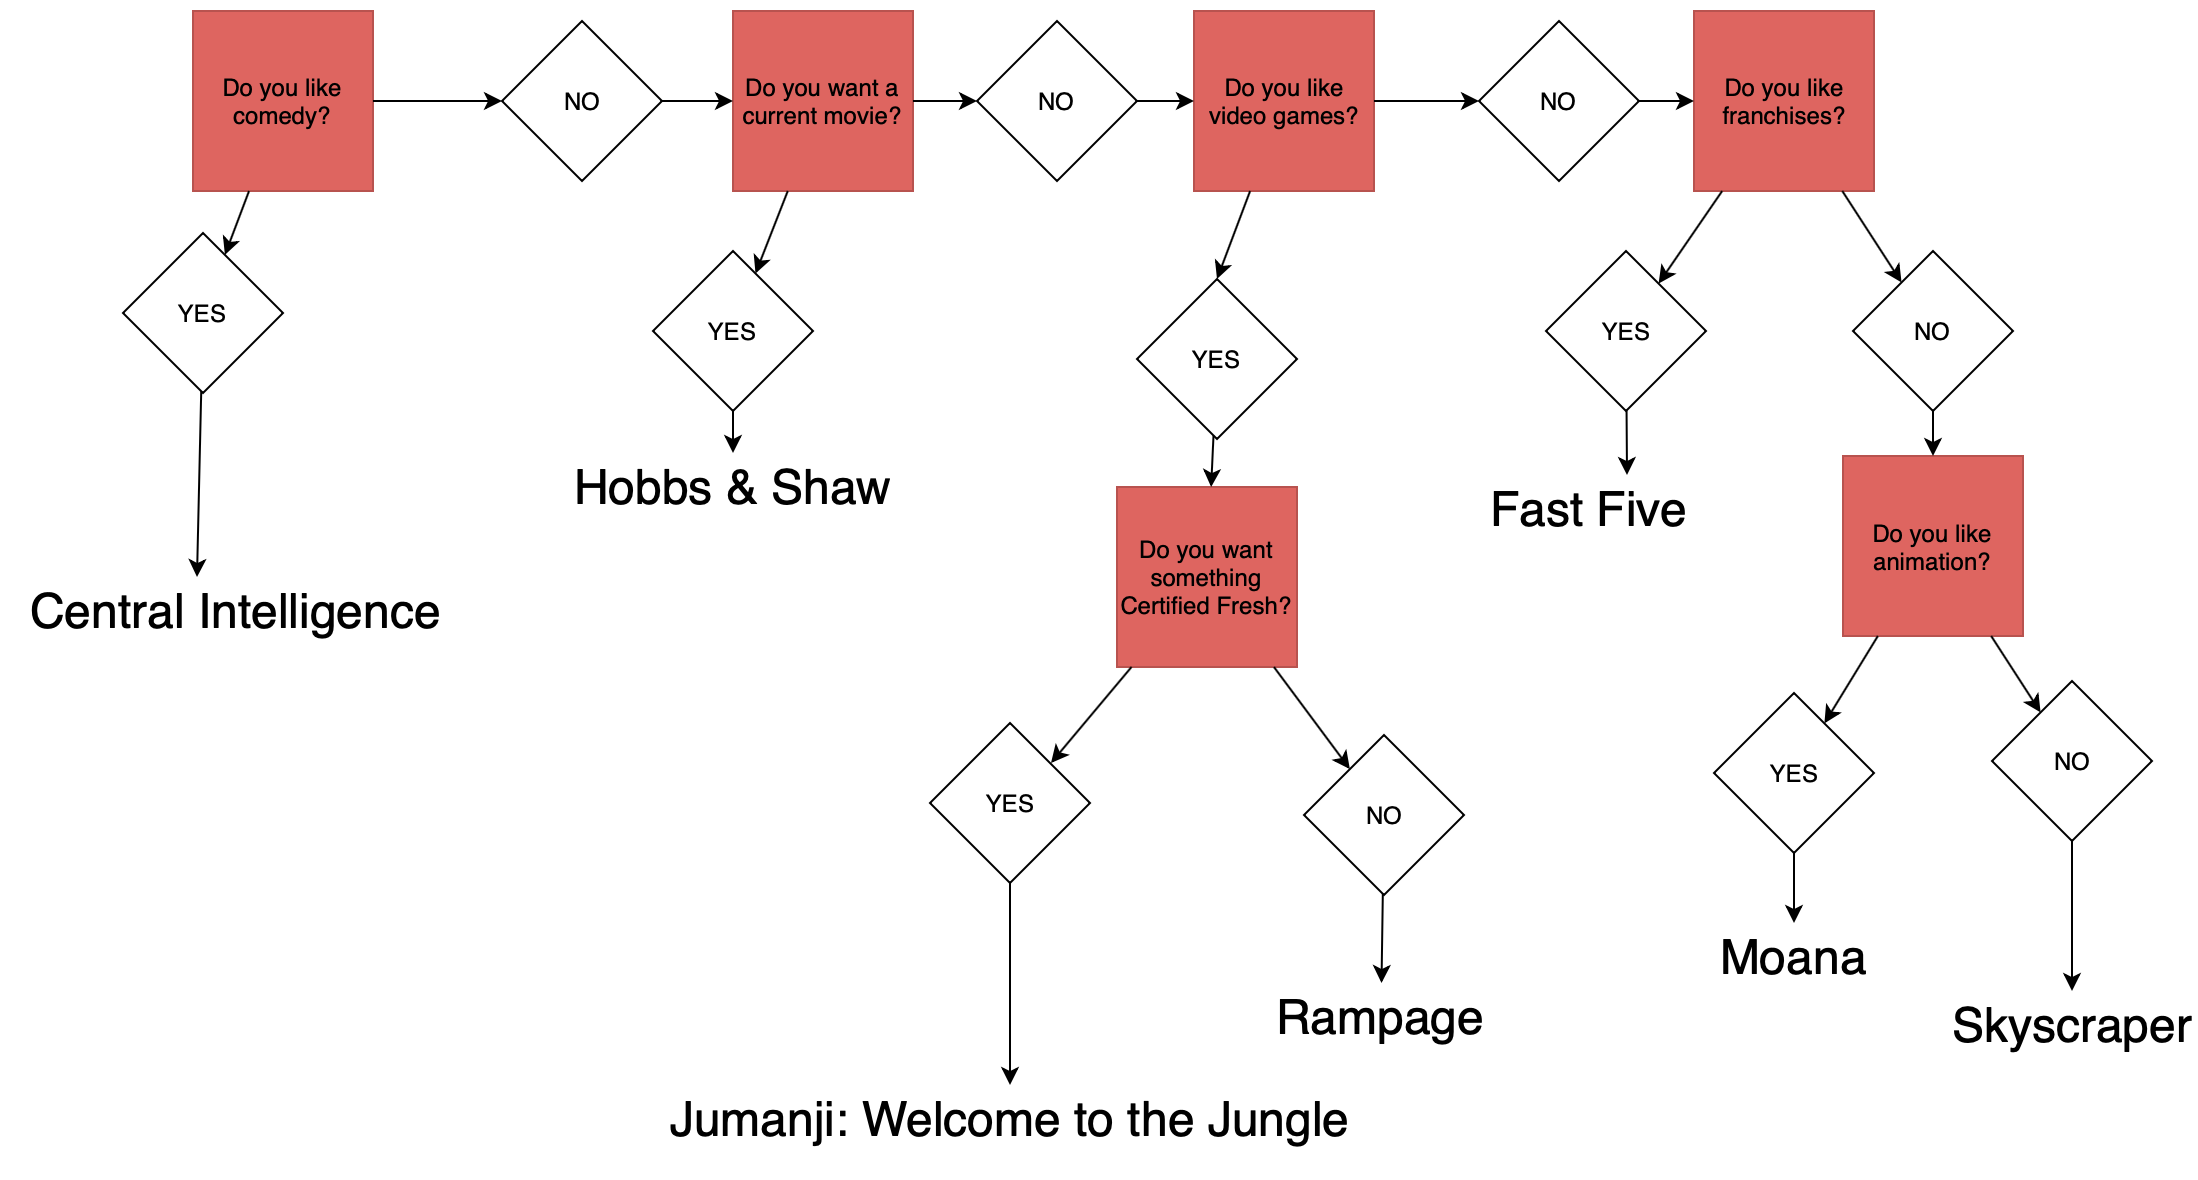
\includegraphics[scale=0.41]{Homework/Homework 05 - Dwayne Johnson Movie Decision Tree.png}
    \caption{Dwayne Johnson movie decision tree}
    \label{fig:movietree}
\end{figure}

\subsection*{Example Compilation and Execution}
\begin{verbatim}
[rzak1@linux1 hw5]$ gcc -Wall movies.c

[rzak1@linux1 hw5]$ ./a.out
Do you like comedy? (y/n) n
Do you want a current movie? (y/n) y
You should see HOBBS & SHAW.

[rzak1@linux1 hw5]$ ./a.out
Do you like comedy? (y/n) y
You should see CENTRAL INTELLIGENCE.

[rzak1@linux1 hw5]$ ./a.out
Do you like comedy? (y/n) n
Do you want a current movie? (y/n) n
Do you like video games? (y/n) y
Do you want something Certified Fresh? (y/n) y
You should see JUMANJI: WELCOME TO THE JUNGLE.

[rzal1@linux1 hw5]$ ./a.out
Do you like comedy? (y/n) n
Do you want a current movie? (y/n) n
Do you like video games? (y/n) n
Do you like franchises? (y/n) n
Do you like animation? (y/n) n
You should see SKYSCRAPER.

[rzak1@linux1 hw5]$ ./a.out
Do you like comedy? (y/n) n
Do you want a current movie? (y/n) n
Do you like video games? (y/n) n
Do you like franchises? (y/n) y
You should see FAST FIVE.
\end{verbatim}

\subsection*{Starter Code}
\begin{verbatim}
/**************************************
** File:  movies.c
** Author: <studentName>
** Date:  10/19/21
** E-mail: <username>@umbc.edu
**
** This file contains the main program for Homework 5.
** This program interacts with a user to suggest a
** Dwayne Johnson movie to watched based on a simple
** decision tree.
**************************************/

#include<stdio.h>

int main() {
   // Define the variables
    char        /* read in y/Y/n/N answer from the user */
    char        /* read in carriage return, but don't really need to use */

   printf("Do you like comedy? ");
   scanf("%c%c",  );

   if () {
      // What's the first movie in the chart?
   } else {
      printf("Do you want a current movie? ");
      
      // Another scanf() to update the variable

      // More if/else statements
   }

   return 0;
}
\end{verbatim}

\subsection*{Notes}
\begin{enumerate}
    \item Please name your C program ``movies.c''
    \item To read in a single character typed in by the user, use the following: \\
    \texttt{scanf("\%c\%c", \&reply, \&cr);} \\
    where \texttt{reply} and \texttt{cr} were declared as variables of type \texttt{char} earlier. \\
    \texttt{char reply, cr;}
    \begin{itemize}
        \item You have to read in two characters because one you need to capture the carriage return typed by the user, which is stored as \texttt{cr}, and isn't needed by the code except for \texttt{scanf()}.
    \end{itemize}
    \item After you read in the character typed in by the user, you can check if the user types a lower case ``y'' or upper case ``Y'' by using: \\
    \texttt{if (reply == `Y' || reply == `y')}
    \begin{itemize}
        \item You may assume that if the user did not type a ``y'' or ``Y'', that they meant \texttt{no}.
    \end{itemize}
    \item You will need several nested levels of \texttt{if} statements similar to Classwork 5. You \textbf{must} indent your program, or you'll be horribly lost.
    \begin{itemize}
        \item If you ask someone to debug an unintented program, it's perfectly reasonable for that person to ask for it to be indented before looking at it.
        \item One way to avoid messing up your braces and indentation is to type in the braces as soon as you type in your \texttt{if} condition. That is, first type in:
        \begin{verbatim}
if (reply == `Y' || reply == `y') {

} else {

}
        \end{verbatim}Then go back and fill in the appropriate areas.
    \end{itemize}
\end{enumerate}

\newpage
\section*{Grading Rubric}
\begin{itemize}
    \item Header comments: 2 points
    \item Body comments: 3 points
    \item Compiles: 40 points
    \item Correct logic: 50 points
    \item Allows y/Y/n/N: 5 points
\end{itemize}

\section*{What to Submit}
\paragraph{}Use the \texttt{script} command to record yourself compiling your program and running your program five times using different search criteria (i.e. different combinations of y and n) each time. Your test runs should result in 5 different movies being recommended. Use \texttt{exit} to terminate the recording. Only record yourself compiling and running your program. \underline{DO NOT} record yourself editing your program. If you mistakenly start up \texttt{nano}, while running script, just exit from script and start over. (The new typescript file will overwrite the old one.)

\paragraph{}When you are done, check the contents of your typescript file. Make sure it does not include you editing your program. Then submit your program and typescript file.
\begin{verbatim}
[rzak1@linux1 hw5]$ cat typescript
NOTE: The contents of your file should display here.
[rzak1@linux1 hw5]$ submit cmsc104_rzak1 hw5 movies.c typescript
\end{verbatim}

\subsection*{Verify Submission}
\paragraph{}If you \textit{think} you submitted the assignment, but the \texttt{submitls} command doesn't show you your file names, then the files were \textbf{not} submitted and no grade will be given.
\begin{verbatim}
[rzak1@linux1 hw5]$ submitls cmsc104_rzak1 hw5
\end{verbatim}

\end{document}